\documentclass[12pt]{article}

\usepackage{amsmath, mathtools}
\usepackage{amsfonts}
\usepackage{amssymb}
\usepackage{graphicx}
\usepackage{colortbl}
\usepackage{xr}
\usepackage{hyperref}
\usepackage{longtable}
\usepackage{xfrac}
\usepackage{tabularx}
\usepackage{float}
\usepackage{siunitx}
\usepackage{booktabs}
\usepackage{caption}
\usepackage{pdflscape}
\usepackage{afterpage}
\usepackage{placeins}
<<<<<<< HEAD
\usepackage{amsthm,letltxmacro,changepage}
=======
>>>>>>> 8c0ee09dbf167771409ef793ed6ecd7b625b452d
\usepackage[shortlabels]{enumitem}

\usepackage[round]{natbib}
\usepackage{multirow}
\usepackage{float}

%\usepackage{refcheck}

\hypersetup{
    bookmarks=true,         % show bookmarks bar?
    colorlinks=true,        % false: boxed links; true: colored links
    linkcolor=red,          % color of internal links (change box color with linkbordercolor)
    citecolor=green,        % color of links to bibliography
    filecolor=magenta,      % color of file links
    urlcolor=cyan           % color of external links
}

%% Comments

\usepackage{color}

\newif\ifcomments\commentstrue %displays comments
%\newif\ifcomments\commentsfalse %so that comments do not display

\ifcomments
\newcommand{\authornote}[3]{\textcolor{#1}{[#3 ---#2]}}
\newcommand{\todo}[1]{\textcolor{red}{[TODO: #1]}}
\else
\newcommand{\authornote}[3]{}
\newcommand{\todo}[1]{}
\fi

\newcommand{\wss}[1]{\authornote{blue}{SS}{#1}} 
\newcommand{\plt}[1]{\authornote{magenta}{TPLT}{#1}} %For explanation of the template
\newcommand{\an}[1]{\authornote{cyan}{Author}{#1}}

%% Common Parts

\newcommand{\progname}{Software Eng} % PUT YOUR PROGRAM NAME HERE
\newcommand{\authname}{Team \#, Team Name
\\ Student 1 Matthew Collard
\\ Student 2 Sam Gorman
\\ Student 3 Ethan Kannampuzha
\\ Student 4 Kieran Gara} % AUTHOR NAMES                  

\usepackage{hyperref}
    \hypersetup{colorlinks=true, linkcolor=blue, citecolor=blue, filecolor=blue,
                urlcolor=blue, unicode=false}
    \urlstyle{same}
                                


% For easy change of table widths
\newcommand{\colZwidth}{1.0\textwidth}
\newcommand{\colAwidth}{0.13\textwidth}
\newcommand{\colBwidth}{0.82\textwidth}
\newcommand{\colCwidth}{0.1\textwidth}
\newcommand{\colDwidth}{0.05\textwidth}
\newcommand{\colEwidth}{0.8\textwidth}
\newcommand{\colFwidth}{0.17\textwidth}
\newcommand{\colGwidth}{0.5\textwidth}
\newcommand{\colHwidth}{0.28\textwidth}

% Used so that cross-references have a meaningful prefix
\newcounter{defnum} %Definition Number
\newcommand{\dthedefnum}{GD\thedefnum}
\newcommand{\dref}[1]{GD\ref{#1}}
\newcounter{datadefnum} %Data definition Number
\newcommand{\ddthedatadefnum}{DD\thedatadefnum}
\newcommand{\ddref}[1]{DD\ref{#1}}
\newcounter{theorynum} %Theory Number
\newcommand{\tthetheorynum}{T\thetheorynum}
\newcommand{\tref}[1]{T\ref{#1}}
\newcounter{tablenum} %Table Number
\newcommand{\tbthetablenum}{T\thetablenum}
\newcommand{\tbref}[1]{TB\ref{#1}}
\newcounter{assumpnum} %Assumption Number
\newcommand{\atheassumpnum}{P\theassumpnum}
\newcommand{\aref}[1]{A\ref{#1}}
\newcounter{goalnum} %Goal Number
\newcommand{\gthegoalnum}{P\thegoalnum}
\newcommand{\gsref}[1]{GS\ref{#1}}
\newcounter{instnum} %Instance Number
\newcommand{\itheinstnum}{IM\theinstnum}
\newcommand{\iref}[1]{IM\ref{#1}}
\newcounter{reqnum} %Requirement Number
\newcommand{\rthereqnum}{P\thereqnum}
\newcommand{\rref}[1]{R\ref{#1}}
\newcounter{nfrnum} %NFR Number
\newcommand{\rthenfrnum}{NFR\thenfrnum}
\newcommand{\nfrref}[1]{NFR\ref{#1}}
\newcounter{lcnum} %Likely change number
\newcommand{\lthelcnum}{LC\thelcnum}
\newcommand{\lcref}[1]{LC\ref{#1}}

\usepackage{fullpage}

\newcommand{\deftheory}[9][Not Applicable]
{
\newpage
\noindent \rule{\textwidth}{0.5mm}

\paragraph{RefName: } \textbf{#2} \phantomsection 
\label{#2}

\paragraph{Label:} #3

\noindent \rule{\textwidth}{0.5mm}

\paragraph{Equation:}

#4

\paragraph{Description:}

#5

\paragraph{Notes:}

#6

\paragraph{Source:}

#7

\paragraph{Ref.\ By:}

#8

\paragraph{Preconditions for \hyperref[#2]{#2}:}
\label{#2_precond}

#9

\paragraph{Derivation for \hyperref[#2]{#2}:}
\label{#2_deriv}

#1

\noindent \rule{\textwidth}{0.5mm}

}

\begin{document}

\title{Software Requirements Specification for \progname: Mac AR}
\author{\authname}
\date{\today}

\maketitle

~\newpage

\pagenumbering{roman}

\tableofcontents

~\newpage

\begin{table}[hp]
	\caption{Revision History} \label{TblRevisionHistory}
	\begin{tabularx}{\textwidth}{llX}
		\toprule
		\textbf{Date}      & \textbf{Developer(s)} & \textbf{Change}                                                                    \\
		\midrule
		September 26, 2023 & Matthew and Sam               & Initial changes to the project                                                             \\
            September 26, 2023 & Matthew & Initial NFR changes \\
            September 28, 2023 & All & General format editing and addition of the Use Case Diagram\\
            September 29, 2023 & Matthew & Addition of Use cases 1-5 and related functional requirements\\
            September 29, 2023 & Kieran & Addition of Use cases 5-10 and related functional requirements\\
            September 29, 2023 & Ethan & Added Read-Made Products section to Project Issues\\
            September 30, 2023 & Ethan & Completed rest of sections in Project Issues\\
            October 1, 2023 & Sam & Filled out sections 1, 6\\
<<<<<<< HEAD
            October 6, 2023 & All & Group worked on traceability matrix and finishing rest of SRS\\  
=======
>>>>>>> 8c0ee09dbf167771409ef793ed6ecd7b625b452d
		\bottomrule
	\end{tabularx}
\end{table}

\newpage

\pagenumbering{arabic}

This document describes the requirements for Mac-AR. The template for the Software Requirements
Specification (SRS) is a subset of the Volere template~\citep{RobertsonAndRobertson2012}. If you
make further modifications to the template, you should explicitly state what modifications were
made.

\section{Project Drivers}

This section will give a general overview of the motivation behind creating Mac-AR, along with what constraints it needs to be created within. 

\subsection{The Purpose of the Project}
In the modern world, it has become increasingly harder to meet new people and form connections with others. This has become especially true in recent years, with the pandemic isolating people even further. Mac-AR aims to solve this by providing a fun, interactive means to cooperate with others and form new connections. As a team, users will be able to work alongside people they already know and strangers around the world to solve interesting puzzles, either outside or from the comfort of their own home. 

\subsection{The Stakeholders}
The following groups and individuals are the reason for the existence of Mac-AR. 

\subsubsection{The Client}
Dr Irene Yuan is the sole client for the project, requesting that the tool be made. She will act as the point of contact during development and ensure that the final result is in line with what was envisioned. 

\subsubsection{The Users}
The users are the ones who will be using the tool and building connections with others. The main user base is intended to be young adults, roughly ages 18-30, who enjoy games and are moderately comfortable using technology.

\subsection{Mandated Constraints}
The project will be developed and released within the following constraints. 

\subsubsection{Solution Constraints} \label{SolutionConstraints}
\emph{Description:} The product shall be built as a mobile application.\\
\emph{Rationale:} The supervisor wants the application to be a mobile application, as to ensure the largest freedom to the users for where and how the product will be used.\\
\emph{Fit Criterion:} The product shall be written using Unity engine.\\

\noindent
<<<<<<< HEAD
\emph{Description:} The product shall be able to function on a variety of mobile devices, using both iOS and Android.\\
\emph{Rationale:} To provide service to the widest array of users, the most popular phone brands, and by extension their operating systems, need to be supported.\\
\emph{Fit Criterion:} The product shall be tested to function on popular mobile devices using iOS and Android, specifically 
\begin{itemize}
	\item Samsung S20 FE 5G
    \item Motorolla G7 Power
    \item Google Pixel 7
    \item iPhone Special Edition 2020
\end{itemize}
=======
\emph{Description:} The product shall be able to function on a variety of mobile devices, such as iPhones and Androids.\\
\emph{Rationale:} To provide service to the widest array of users, the most popular phone brands, and by extension their operating systems, need to be supported.\\
\emph{Fit Criterion:} The product shall be tested to function mobile applications, which includes the following devices:
\begin{itemize}
	\item iPhone SE
	\item iPhone XR
	\item iPhone 12 Pro
	\item Pixel 5
	\item Samsung Galaxy S8+
	\item Samsung Galaxy S20 Ultra
	\item iPad Air
	\item iPad Mini
	\item Surface Pro 7
	\item Surface Duo
	\item Galaxy Fold
	\item Samsung Galaxy A51/71
	\item Nest Hub
	\item Nest Hub Max
\end{itemize}
However, due to timing constraints, testing will only be run on the most popular devices. This would consist of the iPhone, Pixel, and Samsung phones, as well as iPad and Galaxy tablets. For iPhone, which is much more restrictive with backwards compatibility, the most recent IOS versions will be tested, namely 15, 16, and 17.
>>>>>>> 8c0ee09dbf167771409ef793ed6ecd7b625b452d

\subsubsection{Implementation Environment of the Current System}
As outlined in section \ref{SolutionConstraints}, the tool will need to be developed for execution on modern mobile devices. There are currently no constraints on the server side of the project, although that may need to be revised as the tool grows in scope. 

\subsubsection{Partner or Collaborative Applications}
In the current design of the product, there are no partner or collaborative applications that will
work along with the product. Therefore, there are no partner or collaborative constraints.

\subsubsection{Off-the-Shelf Software}
The following off-the-shelf software will be utilized:
\begin{itemize}
	\item Unity, along with its available libraries for AR app development and communication 
        \item Visual Studio, for development
\end{itemize}

\subsubsection{Anticipated Workplace Environment}
The anticipated workplace environment will be intentionally broad. The product can be used from anywhere the user has access to a mobile device and internet to run the application, with no limits on being indoors or outdoors. 

\subsubsection{Schedule Constraints}
The general document and development milestone constraints are as follows:
\begin{table}[H]
	\centering
	\caption{Schedule Constraints}
	\vspace{5pt}
	\begin{tabular}{|p{0.3\textwidth}|p{0.6\textwidth}|}
		\hline
		\textbf{Date}   & \textbf{Deliverable}               \\
		\hline
		Sept 25, 2023    & Problem Statement \\
        \hline
		Sept 25, 2023    & Development Plan \\
        \hline
		Oct 5, 2023    & Requirements Document \\
        \hline
		Oct 20, 2023    & Hazard Analysis \\
		\hline
		Nov 3, 2023     & Verification and Validation Plan   \\
		\hline
		Nov 13-24, 2023 & Proof of Concept Demo              \\
		\hline
		Jan 17, 2024    & Design Document                    \\
		\hline
		Feb 5-16, 2024  & Revision 0 Demo                    \\
		\hline
		Mar 6, 2024     & Verification and Validation Report \\
		\hline
		Mar 18-29, 2024 & Final Demo (Rev 1)                 \\
		\hline
		Apr 4, 2024     & Final Documentation                \\
		\hline
	\end{tabular}
\end{table}

\noindent
As a general constraint applied on top of all of these, all work should be done a few days in advance to allow for time to review. 

\subsubsection{Budget Constraints}
The project has no monetary budget. If there are any necessary purchases for development, the cost
shall be paid by the project members and reimbursed by the supervisor. Furthermore, these purchases
may not exceed \$750.

\subsubsection{Enterprise Constraints}
The project currently has no enterprise constraints. 

\subsection{Naming Conventions and Terminology}

\renewcommand{\arraystretch}{1.2}
\begin{tabular}{l l} 
  \toprule		
  \textbf{Symbol} & \textbf{description}\\
  \midrule 
  A & Assumption\\
  AR & Augmented Reality\\
  DD & Data Definition\\
  GD & General Definition\\
  GPS & Global Positioning System\\
  GS & Goal Statement\\
  IM & Instance Model\\
  LC & Likely Change\\
  PS & Physical System Description\\
  R & Requirement\\
  SRS & Software Requirements Specification\\
  RS & Required Skill\\
  \progname{} & Software Engineering\\
  TM & Theoretical Model\\
  VR & Virtual Reality\\
  XR & Extended Reality\\
  \bottomrule
\end{tabular}\\

\subsection{Relevant Facts and Assumptions}
The product will be developed under the following assumptions.

\subsubsection{User Assumptions}
\begin{itemize}
    \item [A1] Users will have a connection to the internet for the duration of the time that they are actively using the app. 
    \item [A2] The user will provide consent for the app to access the camera on the device which is running the app. 
    \item [A3] The user will provide the app to access locations services and track where the user is while actively using the app. 
\end{itemize}

\subsubsection{Device Assumptions}
\begin{itemize}
    \item [A4] Devices will only have a maximum of one instance of the app running at any given time. 
    \item [A5] The device that the app is running on will have a functional camera. 
    \item [A6] The device that the app is running on will have a functional gyroscope, or equivalent technology to measure device tilt. 
    \item [A7] The device that the app is running on will have a functional GPS, or equivalent technology to measure device location. 
\end{itemize}
<<<<<<< HEAD

\section{Functional Requirements}
The following section will go over the necessary functional requirement information for the project, including use cases. 
\subsection{The Scope of the Work and the Product}
%Not sure where this would go but should have some note that the specific puzzles have not been chosen yet so specifications only given for general puzzle interaction
\subsubsection{Context of the Work}
The context diagram depicted below illustrates the interactions of the system with adjacent
external systems and services.
\begin{figure}[htbp]
\centerline{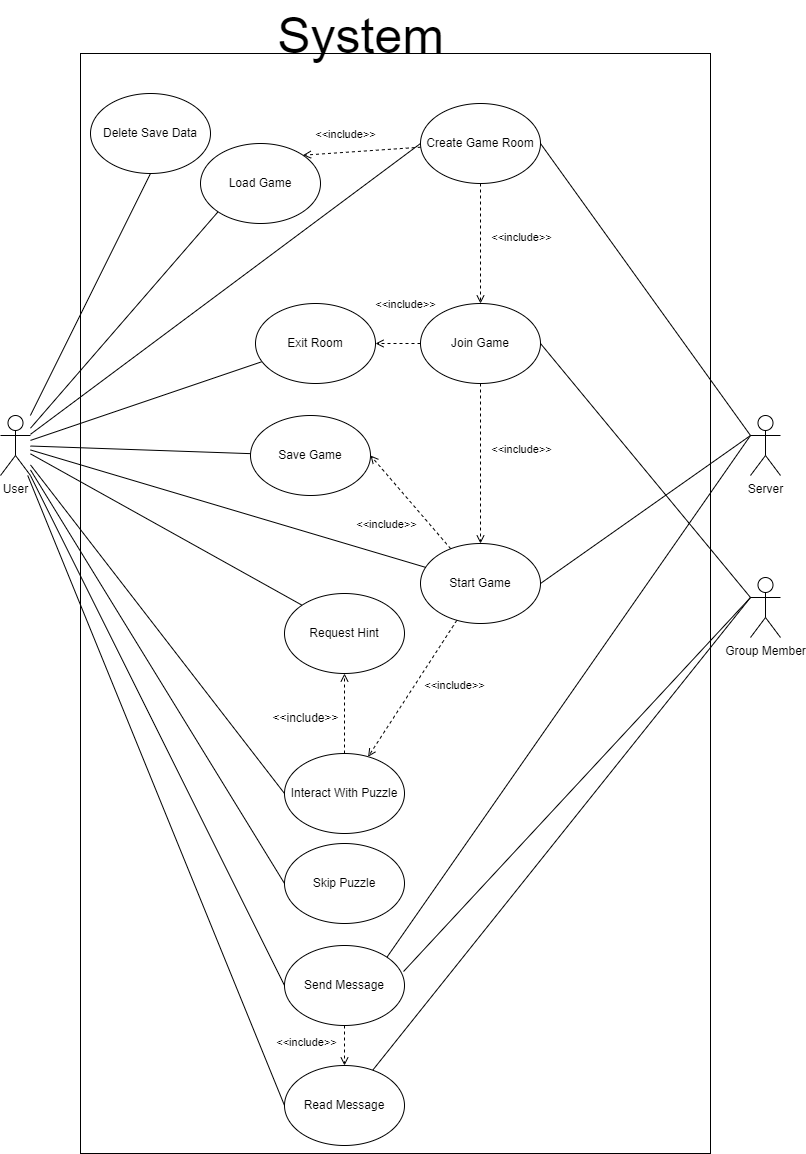
\includegraphics[width=1.05\textwidth]{Capstone/docs/SRS/UseCaseDiagram.png}}
\label{UseCaseDiagram}
\end{figure}

\newpage
\subsubsection{Individual Product Use Cases}

\textbf{Use Case \#1:} User creates a game room\\
\textbf{Trigger:} The user selects the create game room button\\
\textbf{Pre-condition:} N/A\\
\textbf{Outcome:}
\begin{enumerate}
	\item The system creates a room for users to join, and automatically makes the user join the room
    \item The user can choose the length of the game and the settings
	\item The server sends the data of the game room to all the users, to show that the room is available to join, and the capacity of the room, and the current users that have joined the room
\end{enumerate}
\textbf{Use Case \#2:} User Joins Game\\
\textbf{Trigger:} The user selects a room to join that has available capacity\\
\textbf{Pre-condition:} Another user has created a game room\\
\textbf{Outcome:}
\begin{enumerate}
	\item The system links the user to the game room, and decreases the available capacity in the room
    \item The server retrieves the data from the game room and updates the game room for all the users with the new user's name, and decreases the visible room capacity
\end{enumerate}
\textbf{Use Case \#3:} User edits the game room settings\\
\textbf{Trigger:} The user of the game room clicks the edit game settings button\\
\textbf{Pre-condition:} The user created the game room\\
\textbf{Outcome:}
\begin{enumerate}
	\item The system opens the game room settings page
    \item The settings are displayed for the user
    \item The user chooses the settings they want to change
    \item The system updates the game room settings
    \item The server informs the other users of the settings changes
    \item The user closes the settings page
\end{enumerate}
\textbf{Use Case \#4:} User exits the game room\\
\textbf{Trigger:} The user clicks the exit game room button\\
\textbf{Pre-condition:} The user is currently in a game room\\
\textbf{Outcome:}
\begin{enumerate}
	\item The user is removed from the game room
    \item The system updates the information of the game room
    \item The server sends the updated information to each user in the game room
    \item The user is brought back to the main menu
\end{enumerate}
\textbf{Use Case \#5:} User starts the game\\
\textbf{Trigger:} The users in a game room click the start game button\\
\textbf{Pre-condition:} The game room has enough available players\\
\textbf{Outcome:}
\begin{enumerate}
	\item The server launches the game and synchronizes all the user data. 
    \item The user performs a synchronization step to map the room and place the puzzles
    \item The system shows the users the first puzzles
    \item Each user is given a unique view on the puzzles they have available to them
\end{enumerate}
\textbf{Use Case \#6:} User saves game\\
\textbf{Trigger:} The user selects the save game button\\
\textbf{Pre-condition:} There is an active game they are playing in\\
\textbf{Outcome:}
\begin{enumerate}
	\item A local copy of the progress in the game is saved on the user's side
    \item All relevant data on the status of the puzzles is saved
    \item This data can be used to load the game at a later date, and it is safe for users to leave the session
\end{enumerate}
\textbf{Use Case \#7:} User Loads game\\
\textbf{Trigger:} The user hits the load game button and selects the game data they want to load\\
\textbf{Pre-condition:} The user has created a game room, and the user has save data to load\\
\textbf{Outcome:}
\begin{enumerate}
	\item The system reads the user's save data, and when the game is started, the state of the game is loaded
    \item The location of the puzzles might change, but the progress of each puzzle and the total progress of the room is the same as when the game state was saved 
\end{enumerate}
\textbf{Use Case \#8:} User deletes save data\\
\textbf{Trigger:} The user hits delete on their save data\\
\textbf{Pre-condition:} The user has save data\\
\textbf{Outcome:}
\begin{enumerate}
	\item The system deletes the save data from the user's device
    \item The system updates the save data list, and removes that save data from it
\end{enumerate}


\textbf{Use Case \#9:} User interacts with a puzzle\\
\textbf{Trigger:} The user selects a puzzle to attempt\\
\textbf{Pre-condition:} The user has started a puzzle\\
\textbf{Outcome:}
\begin{enumerate} %Doesn't include info about puzzle's impact on other player. Not sure what our intentions are with that.
	\item The system displays an enlarged and interactable version of the puzzle
	\item The user performs an action on the puzzle
	\item The system registers the action, performs any necessary puzzle state changes and displays the new puzzle state to the user    
\end{enumerate}
\textbf{Use Case \#10:} User requests a hint\\
\textbf{Trigger:} The user presses the request hint button\\
\textbf{Pre-condition:} The user has started a puzzle\\
\textbf{Outcome:}
\begin{enumerate}
	\item The system displays the predetermined hint for the associated puzzle
	\item The user reads the hint and presses the button to close the hint
	\item The system closes the hint display.
\end{enumerate}
\textbf{Use Case \#11:} User skips a puzzle\\
\textbf{Trigger:} The user hits the skip button\\
\textbf{Pre-condition:} The user is interacting with a puzzle\\
\textbf{Outcome:}
\begin{enumerate}
	\item The system saves the state of the puzzle and closes the puzzle display, returning to the main scene.
\end{enumerate}
\textbf{Use Case \#12:} User sends a message\\
\textbf{Trigger:} The user presses a communication button\\
\textbf{Pre-condition:} More than one user are in a game room\\
\textbf{Outcome:}
\begin{enumerate}
	\item The system queries the server to determine the users in the room
	\item The system displays the other users in the room to the user
	\item The user selects the desired recipient
        \item The system displays the interface for the user to create the message
        \item The user creates the message and hits the send button
        \item The system uses the server to send the message to the other user's device and to create a message notification on that device. It then notifies the sender that the message has been sent.
\end{enumerate}
\textbf{Use Case \#13:} User reads a message\\
\textbf{Trigger:} The user clicks on a received message notification\\
\textbf{Pre-condition:} The user has received a message\\
\textbf{Outcome:}
\begin{enumerate}
        \item The system removes the message notification and displays the message to the user
	\item The user reads the message, then closes the message display window
	\item The system returns the user to the main game scene.
\end{enumerate}

\subsection{Functional Requirements}
\subsubsection{Create Game Room}
\begin{enumerate}[label=CG\arabic*., series=CreateGame]
    \item The system shall allow the user to create a game room \newline \textbf{Rationale:} The user must be able to group together with other users, creating the game room will allow the users to organize the group.
    \item The system shall allow the user to enter a name for the game room \newline
    \textbf{Rationale:} The users must be able to uniquely identify the game rooms to allow the other users to find the room they want to join in case they have a group they wanted to solve the puzzles with
    \item The system shall allow the user to set the size of the game room \newline
    \textbf{Rationale:} The user should be allowed to limit the size of the room in case they wanted a smaller game rather than a bigger game.
    \item The system shall allow the user to put a password on the game room \newline
    \textbf{Rationale:} The user should be able to allow or disallow any other user from joining except the ones they want in the case they are playing with friends.
    \item The system shall redirect the user to a new screen when in a game room \newline
    \textbf{Rationale: } The users in the room should have a display of the game room and the amount of players in the room etc. 
\end{enumerate}
\subsubsection{Join Game Room}
\begin{enumerate}[label=JG\arabic*., series=JoinGame]
	\item The system shall allow the user to join an existing game room with available capacity \newline 
    \textbf{Rationale:} The user should be able to join a room to group up with other users 
    \item The system shall allow the user to enter a password for the room if another user set a password for the room \newline 
    \textbf{Rationale:} In the case of a game room having a password, the user should be able to have a space to enter the password.
    \item The system shall update the game room information to add another member, and decrease the available capacity\newline 
    \textbf{Rationale:} When a user joins a game room, that information should be updated to let the users users see the status of the room to inform them on which game room to join.
    \item The system shall redirect the user to a new screen upon successfully connecting to a room\newline 
    \textbf{Rationale:} When a user joins the room, they should get redirected to a new page where they can see the information on the current game room and wait for the host to start the game.
\end{enumerate}

\subsubsection{Edit Room Settings}
\begin{enumerate}[label=RS\arabic*., series=EditRoom]
	\item The system shall allow the user that created the game room to edit the settings of the game room\newline 
    \textbf{Rationale:} If a user input the incorrect settings when making a room, the user will have the ability to edit the settings 
    \item The system shall populate all the changeable settings on the user's screen\newline 
    \textbf{Rationale:} The user should be able to see all the settings that are able to be changed
    \item The system shall allow the user to change the password of the room\newline 
    \textbf{Rationale:} The user should be able to change the password of the room to ensure security
    \item The system shall allow the user to change the capacity of the room\newline 
    \textbf{Rationale:} If the user was planning on having a set number of users and decides they want more or less users, they are able to change the capacity
    \item The system shall allow the user to remove other users from the game room\newline 
    \textbf{Rationale:} If the host user decides another user should not be in the game room, they can remove them instead of making a new room
    \item The system shall display the updated settings to the other users in the game room\newline 
    \textbf{Rationale:} When a setting changes the other users in the game room should be able to see the changes in case they will affect them
\end{enumerate}

\subsubsection{Exit Room}
\begin{enumerate}[label=ER\arabic*., series=ExitRoom]
    \item The system shall allow the user leave the existing game room\newline 
    \textbf{Rationale:} If the user does not wish to stay in a game room, the user should be able to leave
    \item The system shall update the game room and display the one less user\newline 
    \textbf{Rationale:} The system should update based on the current number of users
    \item The server shall update all user's screens to show the new amount of users and the updated capacity\newline 
    \textbf{Rationale:} The server should update all the other users on the current capacity and number of users in the game room to inform them of any possible changes
\end{enumerate}


\subsubsection{Start Game}
\begin{enumerate}[label=ST\arabic*., series=StartGame]
	\item The system shall allow the user to start the game\newline 
    \textbf{Rationale:} The users should be able to start the game to play the puzzles
    \item The system shall load all the assets used to play the game\newline 
    \textbf{Rationale:} Loading all the assets at the start of the game will stop pauses during gameplay
    \item The system shall inform the user to complete a calibration step\newline 
    \textbf{Rationale:} AR games require some calibration step to scan the surfaces in the room so objects can be placed with gravity
    \item The system shall determine an order of the puzzles, and which users can see which parts of the puzzles\newline 
    \textbf{Rationale:} In games with more than one puzzle, there needs to be an order to solve the questions. The system will determine a logical order, and assign which users can see which parts of the puzzles.
    \item The system shall display a progress bar based on the current progress on the screen\newline 
    \textbf{Rationale:} The users should have some indicator how close they are to finishing the game
    \item The system shall reveal the available puzzles to the users and commence the game\newline 
    \textbf{Rationale:} The users should be able to view the puzzles they have access to
\end{enumerate}
\subsubsection{Save Game}
\begin{enumerate}[label=SG\arabic*., series=StartGame]
	\item The system shall allow the user to save the game\newline 
    \textbf{Rationale:} Saving the game will allow users to keep the progress on the game they are playing
    \item The system shall take a snapshot of the data available upon hitting save, saving progress on all puzzles and the overall room progress \newline 
    \textbf{Rationale:} If the user wants to load the game in the future they should have all the data required for continuing
    \item The system shall pause the game during the save for the user saving it\newline 
    \textbf{Rationale:} All the game data will be saved based on a point in time, so pausing the user's game to save will allow the game state to remain intact
    \item The system shall allow other users to act during the saving process \newline 
    \textbf{Rationale:} One user saving the game should not stop the other users from continuing playing
    \item After saving, the system shall resume play for the saving user \newline 
    \textbf{Rationale:} The user might want to return to playing after a save
    \item The user shall be allowed to save as many times as they desire, as frequently as they desire aside from the pause during saving. \newline 
    \textbf{Rationale:} There should be no limit on saves in case of any external factors that would effect the game
    \item The system shall store the saved data on the user's device \newline 
    \textbf{Rationale:} Storing the data on the user's device will reduce the stress on the database, the save files should be small in size and it likely won't inconvenience the user
    \item The system shall encode the data such that it is not in its original format and the operation can be reversed \newline 
    \textbf{Rationale:} Encoding the data can reduce the size and prevent users from manually changing the save data and potentially creating issues with the data. 
\end{enumerate}

\subsubsection{Load Game}
\begin{enumerate}[label=LG\arabic*., series=LoadGame]
	\item The system shall allow the user to load an existing save file \newline 
    \textbf{Rationale:} Loading the save files is the purpose for having safe files in the first place
    \item The system shall decode the save file and recall the progress on the saved room\newline 
    \textbf{Rationale:} Decoding the save file makes the data readable by the system
    \item The system shall display the saved data in the game room for all the users to see the progress\newline 
    \textbf{Rationale:} This information will allow the users in the game room to be caught upto date with the progress on the save file
\end{enumerate}

\subsubsection{Delete Save}
\begin{enumerate}[label=DS\arabic*., series=DeleteSave]
	\item The system shall allow to delete the saved game data \newline 
    \textbf{Rationale:} If the user wishes to never load the data, the user can remove it
    \item The system shall remove the saved data from the user's device \newline 
    \textbf{Rationale:} The user's device will no longer hold onto data it won't use
    \item The system shall stop the user from loading the saved game in the future \newline 
    \textbf{Rationale:} Since the saved game data is gone, it should no longer be able to be loaded
\end{enumerate}

\subsubsection{Puzzle Interaction}
    \begin{enumerate}[label=PI\arabic*., series=PuzzleInteract]
        \item The system shall allow users to select a puzzle to attempt from the main scene.\\
        \textbf{Rationale}: The user is shown multiple puzzles on the main scene and must be able to select the one they would like to attempt.
        \item The system shall present the user with an enlarged version of the puzzle once they've selected it.\\
        \textbf{Rationale}: For full scale versions of all puzzles to visible on the main scene, too much of the scene would be obscured. This is resolved by forcing the user to select the puzzle to see the full size puzzle.
        \item The system shall allow users to perform all necessary actions on the puzzle to complete the puzzle.\\
        \textbf{Rationale}: The user must be able to complete the puzzles in order to progress in the game.
        \item The system shall display the new puzzle state after a user performs an action on a puzzle\\
        \textbf{Rationale}: The user must be able to see the results of their actions in order to decide how to proceed with the puzzle
        \item The system shall update the puzzle state of group members cooperating on an updated puzzle\\
        \textbf{Rationale}: When multiple users are cooperating on a puzzle they must be able to see updates caused by the actions of one another.
        \item The system shall notify the user when they have completed a puzzle\\
        \textbf{Rationale}: Users should know when they've completed a puzzle so they know they can move on. A notification at the end of a puzzle can also make completing it more satisfying for the user.
        \item The system shall update the overall room progress when a puzzle is completed\\
        \textbf{Rationale}: The overall room progress must be continuously updated as puzzles are completed so the game can detect when all the puzzles have been completed and the users have accomplished their goal.
    \end{enumerate}
\subsubsection{Hint Request}
    \begin{enumerate}[label=HR\arabic*., series=HintRequest]
        \item The system shall have at least one hint for each puzzle.\\
        \textbf{Rationale}: If a user gets stuck on a puzzle they should have an alternative to giving up on the puzzle.
        \item The system shall have a means of requesting a hint for the puzzle to be displayed.\\
        \textbf{Rationale}: The player must be able to request the hint for the puzzle.
        \item The system shall allow the user to close the hint display\\
        \textbf{Rationale}: The user should not have to keep the hint on the screen, as it may obstruct other functions.
    \end{enumerate}
\subsubsection{Skip Puzzle}
    \begin{enumerate}[label=SP\arabic*., series=SkipPuzzle]
        \item The system shall allow the user to skip a puzzle and return to the main scene.\\
        \textbf{Rationale}: The user should not have to complete a puzzle to attempt a different one. They should be able to leave a puzzle and return to it later.
        \item The system shall save the users progress on a skipped puzzle.\\
        \textbf{Rationale}: If a user skips a puzzle they should be able to return to it without having to start over.
        \item The system shall notify any cooperators on the skipped puzzle that it has been skipped\\
        \textbf{Rationale}: One users work on a puzzle will typically depend on another users work on the puzzle. They must be notified the puzzle has been skipped so they are not waiting on an action from the other user.
    \end{enumerate}
\subsubsection{Send Message}
    \begin{enumerate}[label=SM\arabic*., series=Send Message]
        \item The system shall allow the user to view all the users in the current game room.\\
        \textbf{Rationale}: For the communication system the user must be able to see all the users in the game room to choose who to contact.
        \item The system shall contain an interface that allows the user to compose a message\\
        \textbf{Rationale}: The users must be able to create their own custom messages to allow for optimal communication in puzzles and to create the most realistic social experience.
        \item The system shall allow the user to send a message to any other user in the game room\\
        \textbf{Rationale}: The primary goal of the game is to allow users to have social interaction from a remote setting. All users in the game must be able to interact with one another to complete this goal.
        \item The system shall allow the user to cancel a message before sending it.\\
        \textbf{Rationale}: If a user decides they do not want to send a message they must be able to return to the game without having to send something.
        \item The system shall notify the user once the message has been sent.\\
        \textbf{Rationale}: It is important that the user receive feedback that the message has been sent so there is no uncertainty or confusion for the user.
    \end{enumerate}
\subsubsection{Read Message}
    \begin{enumerate}[label=RM\arabic*., series=ReadMessage]
        \item The system shall notify the user when a new message is received.\\
        \textbf{Rationale}: Communication is core to the game. If a user doesn't know when they receive a message good communication will not be maintained.
        \item The system shall allow the user to view messages.\\
        \textbf{Rationale}: Users must be able to see what other users are trying to communicate to them for social purposes and to complete puzzles.
        \item The system shall allow users to close a message.\\
        \textbf{Rationale}: Users must be able to return to the mains scene after viewing a message to continue game play.
    \end{enumerate}
\subsection{Formal Specification}
$(\forall r \in rooms  | (\sum\limits_{user \in r} 1)  \leq r.roomCapacity)$\\

The users that exist in a room shall be within the capacity of the room

$ (\forall a,b \in puzzles  |  (a \subset b) \implies (a \implies b))$
 
For all the puzzles in the room, if puzzle b depends on a, b will come after a


\section{Non-functional Requirements}
The following section will describe the non-functional requirements of the application.
\subsection{Look and Feel Requirements}
\begin{enumerate}[LF\arabic*.]
	\item The system shall adjust and scale to fit the physical screen size\newline
    \textit{Fit criterion: The display should cover the entire screen and none of it should be cutoff}
	\item The system shall have fonts and colours that will allow users to easily read the text\newline
    \textit{Fit criterion: The system shall abide by the Web Content Accessibility Guidelines (WCAG) 2.1 AA standard~\citep{WCAG2.1}  for fonts and colours}
\end{enumerate}

\subsection{Usability and Humanity Requirements}
\begin{enumerate}[UH\arabic*.]
	\item The system shall be accessible by any supported mobile device\newline
    \textit{Fit criterion: The system should run on the devices listed in solution constraint 1.3.1}
    \item The system shall notify the user if there is no network, or they get disconnected\newline
    \textit{Fit criterion: The system should produce a notification when network connection is lost}
    \item The system shall be able to be navigated by any user\newline
    \textit{Fit criterion: The system shall abide by the WCAG 2.1 AA standard~\citep{WCAG2.1}  for accessibility}
\end{enumerate}
\subsection{Performance Requirements}
\begin{enumerate}[PR\arabic*.]
	\item The system shall respond to user interaction instantaneously as perceived by the user\newline
    \textit{Fit criterion: The system shall respond within 100ms of user interaction}
    \item The system shall be available for users at any time\newline
    \textit{Fit criterion: The system will be accessible 24 hours a day}
\end{enumerate}
\subsection{Operational and Environmental Requirements}
\begin{enumerate}[OE\arabic*.]
    \item The system shall be available on all android and iOS platforms\newline
    \textit{Fit criterion: The system shall be able to be downloaded from the Google Play Store and Apple Store}
\end{enumerate}
\subsection{Maintainability and Support Requirements}
\begin{enumerate}[MS\arabic*.]
    \item The system shall be well documented and kept up to date, and have updated design documents\newline
    \textit{Fit criterion: All changes in the system design are to be reflected in the documents in the GitHub}
    \item The source code shall be well commented for future developers\newline
    \textit{Fit criterion: The system will have author names and dates present in developer code, as well as descriptions of every system module}
\end{enumerate}
\subsection{Security Requirements}
\begin{enumerate}[SR\arabic*.]
    \item The system shall keep user data private\newline
    \textit{Fit criterion: The system shall not make user passwords or IP addresses able to be publicly accessed}
    \item The users will only be allowed to see limited data. Unnecessary data will not be displayed to the user\newline
    \textit{Fit criterion: The system shall only show users any data required in order to play the game}
\end{enumerate}
\subsection{Cultural Requirements}
\begin{enumerate}[CR\arabic*]
    \item The system shall not use any offensive images, text, or sound that could offend any religious or culture groups
    \item The system shall use Canadian English
\end{enumerate}
\subsection{Legal Requirements}
\begin{enumerate}[LR\arabic*]
    \item The system shall not infringe on the rights of any person(s), and shall not use any assets that infringe on copyright claims. When using open source resources, the developers shall give appropriate credit
\end{enumerate}
\subsection{Health and Safety Requirements}
\begin{enumerate}[HS\arabic*]
    \item The system shall give a warning to the user to be aware of their surroundings while using the system, and to not bump into any objects or obstacles in their path
\end{enumerate}

\section{Traceability Matrix}

\begin{table}[H]
\begin{adjustwidth}{-0.1in}{-1in}
\scalebox{0.7}{
\begin{tabular}{c|c|c|c|c|c|c|c|c|c|c|c|c|c|c|c|c|}
\cline{2-17}
                                     & \textbf{LF1} & \textbf{LF2} & \textbf{UH1} & \textbf{UH2} & \textbf{UH3} & \textbf{PR1} & \textbf{PR2} & \textbf{OE1} & \textbf{MR1} & \textbf{MR2} & \textbf{SR1} & \textbf{SR2} & \textbf{CR1} & \textbf{CR2} & \textbf{LR1} & \textbf{HS1}  \\ \hline
\multicolumn{1}{|l|}{\textbf{CG1}}   &      X       &              &       X      &              &       X      &       X      &       X      &       X      &              &              &      X       &      X       &              &      X       &              &               \\ \hline
\multicolumn{1}{|l|}{\textbf{CG2}}   &      X       &      X       &       X      &              &       X      &       X      &       X      &       X      &              &              &              &      X       &      X       &      X       &              &               \\ \hline
\multicolumn{1}{|l|}{\textbf{CG3}}   &      X       &              &       X      &      X       &       X      &       X      &       X      &       X      &              &              &              &      X       &              &      X       &              &               \\ \hline
\multicolumn{1}{|l|}{\textbf{CG4}}   &      X       &      X       &       X      &              &       X      &              &       X      &       X      &              &              &      X       &      X       &              &      X       &              &               \\ \hline
\multicolumn{1}{|l|}{\textbf{CG5}}   &      X       &              &       X      &      X       &       X      &              &              &       X      &              &              &      X       &      X       &              &              &              &               \\ \hline
\multicolumn{1}{|l|}{\textbf{JG1}}   &              &              &              &      X       &              &       X      &       X      &       X      &              &              &              &      X       &              &              &              &               \\ \hline
\multicolumn{1}{|l|}{\textbf{JG2}}   &      X       &      X       &       X      &              &       X      &              &       X      &       X      &              &              &      X       &      X       &              &      X       &              &               \\ \hline
\multicolumn{1}{|l|}{\textbf{JG3}}   &      X       &      X       &       X      &              &       X      &              &              &       X      &              &              &              &              &              &              &              &               \\ \hline
\multicolumn{1}{|l|}{\textbf{JG4}}   &      X       &              &       X      &      X       &       X      &              &              &       X      &              &              &      X       &      X       &              &              &              &               \\ \hline
\multicolumn{1}{|l|}{\textbf{RS1}}   &      X       &      X       &              &              &       x      &              &              &       X      &              &              &              &              &              &      X       &              &               \\ \hline
\multicolumn{1}{|l|}{\textbf{RS2}}   &      X       &      X       &       X      &              &       X      &              &              &       X      &              &              &              &      X       &              &              &              &               \\ \hline
\multicolumn{1}{|l|}{\textbf{RS3}}   &      X       &      X       &       X      &              &       X      &              &              &       X      &              &              &      X       &      X       &              &              &              &               \\ \hline
\multicolumn{1}{|l|}{\textbf{RS4}}   &      X       &      X       &       X      &              &       X      &              &              &       X      &              &              &              &              &              &              &              &               \\ \hline
\multicolumn{1}{|l|}{\textbf{RS5}}   &      X       &      X       &       X      &      X       &       X      &      X       &              &       X      &              &              &      X       &              &      X       &      X       &              &               \\ \hline
\multicolumn{1}{|l|}{\textbf{RS6}}   &      X       &      X       &       X      &              &       X      &              &       X      &       X      &              &              &              &              &              &              &              &               \\ \hline
\multicolumn{1}{|l|}{\textbf{ER1}}   &      X       &      X       &       X      &      X       &       X      &              &       X      &       X      &              &              &      X       &              &              &      X       &              &               \\ \hline
\multicolumn{1}{|l|}{\textbf{ER2}}   &      X       &      X       &       X      &              &       X      &              &              &       X      &              &              &      X       &              &              &      X       &              &               \\ \hline
\multicolumn{1}{|l|}{\textbf{ER3}}   &      X       &      X       &       X      &              &       X      &              &              &       X      &              &              &      X       &              &              &      X       &              &               \\ \hline
\multicolumn{1}{|l|}{\textbf{ST1}}   &      X       &      X       &       X      &              &       X      &      X       &       X      &       X      &              &              &              &              &              &              &              &       X       \\ \hline
\multicolumn{1}{|l|}{\textbf{ST2}}   &              &      X       &       X      &              &              &              &              &       X      &       X      &       X      &              &              &      X       &      X       &      X       &               \\ \hline
\multicolumn{1}{|l|}{\textbf{ST3}}   &      X       &      X       &       X      &              &              &              &              &       X      &              &              &              &              &              &              &              &               \\ \hline
\multicolumn{1}{|l|}{\textbf{ST4}}   &              &              &              &              &              &              &              &       X      &       X      &       X      &              &              &              &              &              &               \\ \hline
\multicolumn{1}{|l|}{\textbf{ST5}}   &      X       &              &       X      &              &              &              &       X      &       X      &              &              &              &              &              &              &              &               \\ \hline
\multicolumn{1}{|l|}{\textbf{ST6}}   &      X       &              &       X      &              &              &              &              &       X      &              &              &              &              &              &              &              &               \\ \hline
\multicolumn{1}{|l|}{\textbf{SG1}}   &      X       &      X       &       X      &       X      &       X      &      X       &       X      &       X      &              &              &      X       &      X       &              &      X       &              &               \\ \hline
\multicolumn{1}{|l|}{\textbf{SG2}}   &              &              &       X      &       X       &             &      X       &       X      &       X      &              &              &      X       &     X        &              &              &              &               \\ \hline
\multicolumn{1}{|l|}{\textbf{SG3}}   &      X       &      X       &       X      &              &              &      X       &       X      &       X      &              &              &              &              &              &              &              &               \\ \hline
\multicolumn{1}{|l|}{\textbf{SG4}}   &      X       &      X       &       X      &              &       X      &      X       &       X      &       X      &              &              &              &              &              &              &              &               \\ \hline
\multicolumn{1}{|l|}{\textbf{SG5}}   &      X       &      X       &       X      &              &              &      X       &       X      &       X      &              &              &              &              &       X      &       X      &              &               \\ \hline
\multicolumn{1}{|l|}{\textbf{SG6}}   &      X       &      X       &       X      &              &       X      &      X       &       X      &       X      &              &              &       X      &              &              &              &              &               \\ \hline
\multicolumn{1}{|l|}{\textbf{SG7}}   &              &              &              &              &              &      X       &       X      &       X      &              &              &       X      &       X      &              &              &              &               \\ \hline
\multicolumn{1}{|l|}{\textbf{SG8}}   &              &              &              &              &              &      X       &       X      &       X      &       X      &       X      &       X      &       X      &              &              &              &               \\ \hline
\multicolumn{1}{|l|}{\textbf{LG1}}   &      X       &      X       &       X      &              &       X      &      X       &       X      &       X      &              &              &              &       X      &       X      &       X      &              &               \\ \hline
\multicolumn{1}{|l|}{\textbf{LG2}}   &              &              &              &              &              &      X       &       X      &       X      &       X      &       X      &       X      &       X      &              &              &              &               \\ \hline
\multicolumn{1}{|l|}{\textbf{LG3}}   &      X       &      X       &       X      &       X      &       X      &      X       &       X      &       X      &              &              &              &              &       X      &       X      &              &               \\ \hline
\multicolumn{1}{|l|}{\textbf{DS1}}   &      X       &      X       &       X      &              &       X      &      X       &       X      &       X      &              &              &       X      &       X      &       X      &       X      &              &               \\ \hline
\multicolumn{1}{|l|}{\textbf{DS2}}   &              &              &       X      &              &              &      X       &              &       X      &       X      &       X      &       X      &       X      &              &              &              &               \\ \hline
\multicolumn{1}{|l|}{\textbf{DS3}}   &              &              &       X      &              &       X      &      X       &              &       X      &              &              &       X      &       X      &       X      &       X      &              &               \\ \hline

\end{tabular}

}
\caption{Traceability Matrix}
    \label{tab:matrix1}
\end{adjustwidth}
\end{table}


\begin{table}[H]
\begin{adjustwidth}{-0.1in}{-1in}
\scalebox{0.7}{
\begin{tabular}{c|c|c|c|c|c|c|c|c|c|c|c|c|c|c|c|c|}
\cline{2-17}
                                     & \textbf{LF1} & \textbf{LF2} & \textbf{UH1} & \textbf{UH2} & \textbf{UH3} & \textbf{PR1} & \textbf{PR2} & \textbf{OE1} & \textbf{MR1} & \textbf{MR2} & \textbf{SR1} & \textbf{SR2} & \textbf{CR1} & \textbf{CR2} &\textbf{LR1} & \textbf{HS1} \\ \hline
\multicolumn{1}{|l|}{\textbf{PI1}}   &      X       &       X      &       X      &       X      &       X      &       X      &       X      &       X      &              &              &              &       X      &       X      &       X      &             &      X       \\ \hline
\multicolumn{1}{|l|}{\textbf{PI2}}   &      X       &       X      &       X      &              &       X      &       X      &       X      &       X      &              &              &       X      &       X      &       X      &       X      &             &      X       \\ \hline
\multicolumn{1}{|l|}{\textbf{PI3}}   &      X       &       X      &       X      &              &       X      &       X      &       X      &       X      &              &              &              &       X      &       X      &       X      &             &              \\ \hline
\multicolumn{1}{|l|}{\textbf{PI4}}   &      X       &       X      &       X      &              &              &       X      &       X      &       X      &              &              &              &       X      &       X      &       X      &             &              \\ \hline
\multicolumn{1}{|l|}{\textbf{PI5}}   &      X       &       X      &       X      &       X      &              &       X      &       X      &       X      &              &              &       X      &       X      &       X      &       X      &             &              \\ \hline
\multicolumn{1}{|l|}{\textbf{PI6}}   &      X       &       X      &       X      &       X      &              &       X      &       X      &       X      &              &              &              &              &       X      &       X      &             &              \\ \hline
\multicolumn{1}{|l|}{\textbf{PI7}}   &      X       &       X      &       X      &       X      &              &       X      &       X      &       X      &              &              &              &              &       X      &       X      &             &              \\ \hline
\multicolumn{1}{|l|}{\textbf{HR1}}   &              &              &              &              &              &              &       X      &       X      &      X       &      X       &       X      &       X      &              &              &      X      &              \\ \hline
\multicolumn{1}{|l|}{\textbf{HR2}}   &      X       &       X      &       X      &       X      &       X      &       X      &       X      &       X      &              &              &              &              &       X      &       X      &             &              \\ \hline
\multicolumn{1}{|l|}{\textbf{HR3}}   &      X       &       X      &              &       X      &       X      &       X      &       X      &       X      &              &              &              &              &       X      &       X      &             &              \\ \hline
\multicolumn{1}{|l|}{\textbf{SP1}}   &      X       &       X      &              &       X      &       X      &       X      &       X      &       X      &              &              &              &              &       X      &       X      &             &              \\ \hline
\multicolumn{1}{|l|}{\textbf{SP2}}   &              &              &              &              &              &       X      &       X      &       X      &      X       &      X       &       X      &       X      &              &              &      X      &              \\ \hline
\multicolumn{1}{|l|}{\textbf{SP3}}   &      X       &       X      &              &       X      &       X      &       X      &       X      &       X      &              &              &              &              &       X      &       X      &             &              \\ \hline
\multicolumn{1}{|l|}{\textbf{SM1}}   &      X       &       X      &       X      &       X      &       X      &              &       X      &       X      &              &              &              &       X      &              &       X      &             &              \\ \hline
\multicolumn{1}{|l|}{\textbf{SM2}}   &      X       &       X      &       X      &       X      &       X      &              &       X      &       X      &              &              &              &       X      &              &       X      &             &              \\ \hline
\multicolumn{1}{|l|}{\textbf{SM3}}   &      X       &       X      &       X      &       X      &       X      &       X      &       X      &       X      &              &              &       X      &       X      &              &       X      &             &              \\ \hline
\multicolumn{1}{|l|}{\textbf{SM4}}   &      X       &       X      &       X      &       X      &       X      &       X      &       X      &       X      &              &              &       X      &       X      &              &       X      &             &              \\ \hline
\multicolumn{1}{|l|}{\textbf{SM5}}   &      X       &       X      &       X      &       X      &              &       X      &       X      &       X      &              &              &       X      &       X      &       X      &       X      &             &              \\ \hline
\multicolumn{1}{|l|}{\textbf{RM1}}   &      X       &       X      &       X      &       X      &       X      &       X      &       X      &       X      &              &              &       X      &       X      &       X      &       X      &             &              \\ \hline
\multicolumn{1}{|l|}{\textbf{RM2}}   &      X       &       X      &       X      &       X      &       X      &       X      &       X      &       X      &              &              &       X      &       X      &       X      &       X      &             &              \\ \hline
\multicolumn{1}{|l|}{\textbf{RM3}}   &      X       &       X      &       X      &       X      &       X      &       X      &       X      &       X      &              &              &       X      &       X      &       X      &       X      &             &              \\ \hline
\end{tabular}

}
\caption{Traceability Matrix}
    \label{tab:matrix2}
\end{adjustwidth}
\end{table}





=======

\section{Functional Requirements}

\subsection{The Scope of the Work and the Product}

\subsubsection{The Current Situation}
%Not sure where this would go but should have some note that the specific puzzles have not been chosen yet so specifications only given for general puzzle interaction
\subsubsection{Context of the Work}
The context diagram depicted below illustrates the interactions of the system with adjacent
external systems and services.
\begin{figure}[htbp]
\centerline{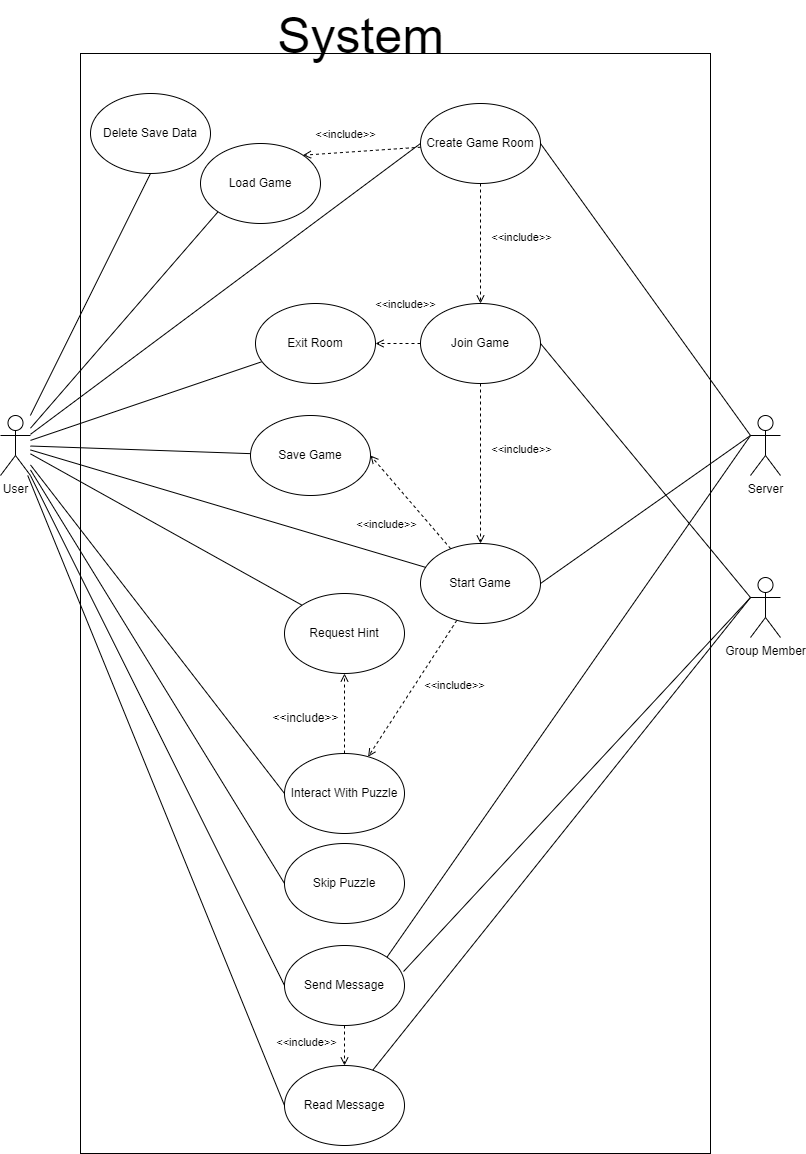
\includegraphics[width=1.05\textwidth]{Capstone/docs/SRS/UseCaseDiagram.png}}
\label{UseCaseDiagram}
\end{figure}

\newpage
\subsubsection{Individual Product Use Cases}

\textbf{Use Case \#1:} User creates a game room\\
\textbf{Trigger:} The user selects the create game room button\\
\textbf{Pre-condition:} N/A\\
\textbf{Outcome:}
\begin{enumerate}
	\item The system creates a room for users to join, and automatically makes the user join the room
    \item The user can choose the length of the game and the settings
	\item The server sends the data of the game room to all the users, to show that the room is available to join, and the capacity of the room, and the current users that have joined the room
\end{enumerate}
\textbf{Use Case \#2:} User Joins Game\\
\textbf{Trigger:} The user selects a room to join that has available capacity\\
\textbf{Pre-condition:} Another user has created a game room\\
\textbf{Outcome:}
\begin{enumerate}
	\item The system links the user to the game room, and decreases the available capacity in the room
    \item The server retrieves the data from the game room and updates the game room for all the users with the new user's name, and decreases the visible room capacity
\end{enumerate}
\textbf{Use Case \#3:} User edits the game room settings\\
\textbf{Trigger:} The user of the game room clicks the edit game settings button\\
\textbf{Pre-condition:} The user created the game room\\
\textbf{Outcome:}
\begin{enumerate}
	\item The system opens the game room settings page
    \item The settings are displayed for the user
    \item The user chooses the settings they want to change
    \item The system updates the game room settings
    \item The server informs the other users of the settings changes
    \item The user closes the settings page
\end{enumerate}
\textbf{Use Case \#4:} User exits the game room\\
\textbf{Trigger:} The user clicks the exit game room button\\
\textbf{Pre-condition:} The user is currently in a game room\\
\textbf{Outcome:}
\begin{enumerate}
	\item The user is removed from the game room
    \item THe system updates the information of the game room
    \item The server sends the updated information to each user in the game room
    \item The user is brought back to the main menu
\end{enumerate}
\textbf{Use Case \#5:} User starts the game\\
\textbf{Trigger:} The users in a game room click the start game button\\
\textbf{Pre-condition:} The game room has enough available players\\
\textbf{Outcome:}
\begin{enumerate}
	\item The server launches the game and synchronizes all the user data. 
    \item The user performs a synchronization step to map the room and place the puzzles
    \item The system shows the users the first puzzles
    \item Each user is given a unique view on the puzzles they have available to them
\end{enumerate}
\textbf{Use Case \#6:} User saves game\\
\textbf{Trigger:} The user selects the save game button\\
\textbf{Pre-condition:} There is an active game they are playing in\\
\textbf{Outcome:}
\begin{enumerate}
	\item A local copy of the progress in the game is saved on the user's side
    \item All relevant data on the status of the puzzles is saved
    \item This data can be used to load the game at a later date, and it is safe for users to leave the session
\end{enumerate}
\textbf{Use Case \#7:} User Loads game\\
\textbf{Trigger:} The user hits the load game button and selects the game data they want to load\\
\textbf{Pre-condition:} The user has created a game room, and the user has save data to load\\
\textbf{Outcome:}
\begin{enumerate}
	\item The system reads the user's save data, and when the game is started, the state of the game is loaded
    \item The location of the puzzles might change, but the progress of each puzzle and the total progress of the room is the same as when the game state was saved 
\end{enumerate}
\textbf{Use Case \#8:} User deletes save data\\
\textbf{Trigger:} The user hits delete on their save data\\
\textbf{Pre-condition:} The user has save data\\
\textbf{Outcome:}
\begin{enumerate}
	\item The system deletes the save data from the user's device
    \item The system updates the save data list, and removes that save data from it
\end{enumerate}


\textbf{Use Case \#9:} User interacts with a puzzle\\
\textbf{Trigger:} The user selects a puzzle to attempt\\
\textbf{Pre-condition:} The user has started a puzzle\\
\textbf{Outcome:}
\begin{enumerate} %Doesn't include info about puzzle's impact on other player. Not sure what our intentions are with that.
	\item The system displays an enlarged and interactable version of the puzzle
	\item The user performs an action on the puzzle
	\item The system registers the action, performs any necessary puzzle state changes and displays the new puzzle state to the user    
\end{enumerate}
\textbf{Use Case \#10:} User requests a hint\\
\textbf{Trigger:} The user presses the request hint button\\
\textbf{Pre-condition:} The user has started a puzzle\\
\textbf{Outcome:}
\begin{enumerate}
	\item The system displays the predetermined hint for the associated puzzle
	\item The user reads the hint and presses the button to close the hint
	\item The system closes the hint display.
\end{enumerate}
\textbf{Use Case \#11:} User skips a puzzle\\
\textbf{Trigger:} The user hits the skip button\\
\textbf{Pre-condition:} The user is interacting with a puzzle\\
\textbf{Outcome:}
\begin{enumerate}
	\item The system saves the state of the puzzle and closes the puzzle display, returning to the main scene.
\end{enumerate}
\textbf{Use Case \#12:} User sends a message\\
\textbf{Trigger:} The user presses a communication button\\
\textbf{Pre-condition:} More than one user are in a game room\\
\textbf{Outcome:}
\begin{enumerate}
	\item The system queries the server to determine the users in the room
	\item The system displays the other users in the room to the user
	\item The user selects the desired recipient
        \item The system displays the interface for the user to create the message
        \item The user creates the message and hits the send button
        \item The system uses the server to send the message to the other user's device and to create a message notification on that device. It then notifies the sender that the message has been sent.
\end{enumerate}
\textbf{Use Case \#13:} User reads a message\\
\textbf{Trigger:} The user clicks on a received message notification\\
\textbf{Pre-condition:} The user has received a message\\
\textbf{Outcome:}
\begin{enumerate}
        \item The system removes the message notification and displays the message to the user
	\item The user reads the message, then closes the message display window
	\item The system returns the user to the main game scene.
\end{enumerate}

\subsection{Functional Requirements}

\subsubsection{Create Game Room}
\begin{enumerate}[label=CG\arabic*., series=CreateGame]
    \item The system shall allow the user to create a game room \newline \textbf{Rationale:} The user must be able to group together with other users, creating the game room will allow the users to organize the group.
    \item The system shall allow the user to enter a name for the room \newline
    \textbf{Rationale:} The users must be able to uniquely identify the game rooms to allow the other users to find the room they want to join in case they have a group they wanted to solve the puzzles with
    \item The system shall allow the user to set the size of the room \newline
    \textbf{Rationale:} The user should be allowed to limit the size of the room in case they wanted a smaller game rather than a bigger game.
    \item The system shall allow the user to put a password on the room \newline
    \textbf{Rationale:} The user should be able to allow or disallow any other user from joining except the ones they want in the case they are playing with friends.
    \item The system shall redirect the user to a new screen when in a room \newline
    \textbf{Rationale: } The users in the room should have a display of the game room and the amount of players in the room etc. 
\end{enumerate}
\subsubsection{Join Game Room}
\begin{enumerate}[label=JG\arabic*., series=JoinGame]
	\item The system shall allow the user to join an existing game room with available capacity \newline 
    \textbf{Rationale:} The user should be able to join a room to group up with other users 
    \item The system shall allow the user to enter a password for the room if another user set a password for the room \newline 
    \textbf{Rationale:} In the case of a game room having a password, the user should be able to have a space to enter the password.
    \item The system shall update the game room information to add another member, and decrease the available capacity\newline 
    \textbf{Rationale:} When a user joins a game room, that information should be updated to let the users users see the status of the room to inform them on which game room to join.
    \item The system shall redirect the user to a new screen upon successfully connecting to a room\newline 
    \textbf{Rationale:} When a user joins the room, they should get redirected to a new page where they can see the information on the current game room and wait for the host to start the game.
\end{enumerate}

\subsubsection{Edit Room Settings}
\begin{enumerate}[label=RS\arabic*., series=EditRoom]
	\item The system shall allow the user that created the game room to edit the settings of the game room\newline 
    \textbf{Rationale:} If a user input the incorrect settings when making a room, the user will have the ability to edit the settings 
    \item The system shall populate all the changeable settings on the user's screen\newline 
    \textbf{Rationale:} The user should be able to see all the settings that are able to be changed
    \item The system shall allow the user to change the password of the room\newline 
    \textbf{Rationale:} The user should be able to change the password of the room to ensure security
    \item The system shall allow the user to change the capacity of the room\newline 
    \textbf{Rationale:} If the user was planning on having a set number of users and decides they want more or less users, they are able to change the capacity
    \item The system shall allow the user to remove other users from the game room\newline 
    \textbf{Rationale:} If the host user decides another user should not be in the game room, they can remove them instead of making a new room
    \item The system shall display the updated settings to the other users in the game room\newline 
    \textbf{Rationale:} When a setting changes the other users in the game room should be able to see the changes in case they will affect them
\end{enumerate}

\subsubsection{Exit Room}
\begin{enumerate}[label=ER\arabic*., series=ExitRoom]
    \item The system shall allow the user leave the existing game room\newline 
    \textbf{Rationale:} If the user does not wish to stay in a game room, the user should be able to leave
    \item The system shall update the game room and display the one less user\newline 
    \textbf{Rationale:} The system should update based on the current number of users
    \item The server shall update all user's screen to show the new amount of users and the updated capacity\newline 
    \textbf{Rationale:} The server should update all the other users on the current capacity and number of users in the game room to inform them of any possible changes
\end{enumerate}


\subsubsection{Start Game}
\begin{enumerate}[label=ST\arabic*., series=StartGame]
	\item The system shall allow the user to start the game\newline 
    \textbf{Rationale:} The users should be able to start the game to play the puzzles
    \item The system shall load all the assets used to play the game\newline 
    \textbf{Rationale:} Loading all the assets at the start of the game will stop pauses during gameplay
    \item The system shall inform the user to complete a calibration step\newline 
    \textbf{Rationale:} AR games require some calibration step to scan the surfaces in the room so objects can be placed with gravity
    \item The system shall determine an order of the puzzles, and which users can see which parts of the puzzles\newline 
    \textbf{Rationale:} In games with more than one puzzle, there needs to be an order to solve the questions. The system will determine a logical order, and assign which users can see which parts of the puzzles.
    \item The system shall display a progress bar based on the current progress on the screen\newline 
    \textbf{Rationale:} The users should have some indicator how close they are to finishing the game
    \item The system shall reveal the available puzzles to the users and commence the game\newline 
    \textbf{Rationale:} The users should be able to view the puzzles they have access to
\end{enumerate}
\subsubsection{Save Game}
\begin{enumerate}[label=SG\arabic*., series=StartGame]
	\item The system shall allow the user to save the game\newline 
    \textbf{Rationale:} Saving the game will allow users to keep the progress on the game they are playing
    \item The system shall save all the relevant data needed for reloading the game \newline 
    \textbf{Rationale:} If the user wants to load the game in the future they should have all the data required for continuing
    \item The system will pause the game during the save for the user saving it, and take a screenshot of the data available upon hitting save \newline 
    \textbf{Rationale:} All the game data will be saved based on a point in time, so pausing the user's game to save will allow the game state to remain intact
    \item The system shall allow other users to act during the saving process \newline 
    \textbf{Rationale:} One user saving the game should not stop the other users from continuing playing
    \item After saving, the system shall resume play for the saving user \newline 
    \textbf{Rationale:} The user might want to return to playing after a save
    \item The user shall be allowed to save as many times as they desire, as frequently as they desire. \newline 
    \textbf{Rationale:} There should be no limit on saves in case of any external factors that would effect the game
    \item The system shall put the saved data on the user's device \newline 
    \textbf{Rationale:} Storing the data on the user's device will reduce the stress on the database, the save files should be small in size and it likely won't inconvenience the user
    \item The system shall encode the data \newline 
    \textbf{Rationale:} Encoding the data can reduce the size and prevent users from manually changing the save data and potentially creating issues with the data. 
\end{enumerate}

\subsubsection{Load Game}
\begin{enumerate}[label=LG\arabic*., series=LoadGame]
	\item The system shall allow the user to load an existing save file \newline 
    \textbf{Rationale:} Loading the save files is the purpose for having safe files in the first place
    \item The system shall decode the save file and recall the progress on the saved room\newline 
    \textbf{Rationale:} Decoding the save file makes the data readable by the system
    \item The system shall display the saved data in the game room for all the users to see the progress\newline 
    \textbf{Rationale:} This information will allow the users in the game room to be caught upto date with the progress on the save file
\end{enumerate}

\subsubsection{Delete Save}
\begin{enumerate}[label=DS\arabic*., series=DeleteSave]
	\item The system shall allow to delete the saved game data \newline 
    \textbf{Rationale:} If the user wishes to never load the data, the user can remove it
    \item The system shall remove the saved data from the user's device \newline 
    \textbf{Rationale:} The user's device will no longer hold onto data it won't use
    \item The system shall stop the user from loading the saved game in the future \newline 
    \textbf{Rationale:} Since the saved game data is gone, it should no longer be able to be loaded
\end{enumerate}

\subsubsection{Puzzle Interaction}
    \begin{enumerate}[label=PI\arabic*., series=PuzzleInteract]
        \item The system shall allow users to select a puzzle to attempt from the main scene.\\
        \textbf{Rationale}: The user is shown multiple puzzles on the main scene and must be able to select the one they would like to attempt.
        \item The system shall present the user with an enlarged version of the puzzle once they've selected it.\\
        \textbf{Rationale}: For full scale versions of all puzzles to visible on the main scene, too much of the scene would be obscured. This is resolved by forcing the user to select the puzzle to see the full size puzzle.
        \item The system shall allow users to perform all necessary actions on the puzzle to complete the puzzle.\\
        \textbf{Rationale}: The user must be able to complete the puzzles in order to progress in the game.
        \item The system shall display the new puzzle state after a user performs an action on a puzzle\\
        \textbf{Rationale}: The user must be able to see the results of their actions in order to decide how to proceed with the puzzle
        \item The system shall update the puzzle state of group members cooperating on an updated puzzle\\
        \textbf{Rationale}: When multiple users are cooperating on a puzzle they must be able to see updates caused by the actions of one another.
        \item The system shall notify the user when they have completed a puzzle\\
        \textbf{Rationale}: Users should know when they've completed a puzzle so they know they can move on. A notification at the end of a puzzle can also make completing it more satisfying for the user.
        \item The system shall update the overall room progress when a puzzle is completed\\
        \textbf{Rationale}: The overall room progress must be continuously updated as puzzles are completed so the game can detect when all the puzzles have been completed and the users have accomplished their goal.
    \end{enumerate}
\subsubsection{Hint Request}
    \begin{enumerate}[label=HR\arabic*., series=HintRequest]
        \item The system shall have at least one hint for each puzzle.\\
        \textbf{Rationale}: If a user gets stuck on a puzzle they should have an alternative to giving up on the puzzle.
        \item The system shall have a means of requesting a hint for the puzzle to be displayed.\\
        \textbf{Rationale}: The player must be able to request the hint for the puzzle.
        \item The system shall allow the user to close the hint display\\
        \textbf{Rationale}: The user should not have to keep the hint on the screen, as it may obstruct other functions.
    \end{enumerate}
\subsubsection{Skip Puzzle}
    \begin{enumerate}[label=SP\arabic*., series=SkipPuzzle]
        \item The system shall allow the user to skip a puzzle and return to the main scene.\\
        \textbf{Rationale}: The user should not have to complete a puzzle to attempt a different one. They should be able to leave a puzzle and return to it later.
        \item The system shall save the users progress on a skipped puzzle.\\
        \textbf{Rationale}: If a user skips a puzzle they should be able to return to it without having to start over.
        \item The system shall notify any cooperators on the skipped puzzle that it has been skipped\\
        \textbf{Rationale}: One users work on a puzzle will typically depend on another users work on the puzzle. They must be notified the puzzle has been skipped so they are not waiting on an action from the other user.
    \end{enumerate}
\subsubsection{Send Message}
    \begin{enumerate}[label=SM\arabic*., series=Send Message]
        \item The system shall allow the user to view all the users in the current game room.\\
        \textbf{Rationale}: For the communication system the user must be able to see all the users in the game room to choose who to contact.
        \item The system shall contain an interface that allows the user to compose a message\\
        \textbf{Rationale}: The users must be able to create their own custom messages to allow for optimal communication in puzzles and to create the most realistic social experience.
        \item The system shall allow the user to send a message to any other user in the game room\\
        \textbf{Rationale}: The primary goal of the game is to allow users to have social interaction from a remote setting. All users in the game must be able to interact with one another to complete this goal.
        \item The system shall allow the user to cancel a message before sending it.\\
        \textbf{Rationale}: If a user decides they do not want to send a message they must be able to return to the game without having to send something.
        \item The system shall notify the user once the message has been sent.\\
        \textbf{Rationale}: It is important that the user receive feedback that the message has been sent so there is no uncertainty or confusion for the user.
    \end{enumerate}
\subsubsection{Read Message}
    \begin{enumerate}[label=RM\arabic*., series=ReadMessage]
        \item The system shall notify the user when a new message is received.\\
        \textbf{Rationale}: Communication is core to the game. If a user doesn't know when they receive a message good communication will not be maintained.
        \item The system shall allow the user to view messages.\\
        \textbf{Rationale}: Users must be able to see what other users are trying to communicate to them for social purposes and to complete puzzles.
        \item The system shall allow users to close a message.\\
        \textbf{Rationale}: Users must be able to return to the mains scene after viewing a message to continue game play.
    \end{enumerate}
\subsection{Formal Specification}
$(\exists a \in \text{users} \And \exists r \in \text{room} \And c=r.capacity | \sum a \in r \leq c ) \Rightarrow
	true)$\\
The users that exist in a room shall be within the capacity of the room


\section{Non-functional Requirements}

\subsection{Look and Feel Requirements}
\begin{enumerate}[LF\arabic*.]
	\item The system shall adjust and scale to fit the physical screen size
	\item The system shall have fonts and colours that will allow users to easily read the text
\end{enumerate}

\subsection{Usability and Humanity Requirements}
\begin{enumerate}[UH\arabic*.]
	\item The system shall be accessible by any supported mobile device
        \item The system shall notify the user if there is no network, or they get disconnected
        \item The system shall be able to be navigated by any user
\end{enumerate}
\subsection{Performance Requirements}
\begin{enumerate}[PR\arabic*.]
	\item The system shall respond to user interaction within 100ms
        \item The system shall be available for users at any time
\end{enumerate}
\subsection{Operational and Environmental Requirements}
\begin{enumerate}[OE\arabic*.]
    \item The system shall be available on all android and iOS platforms
\end{enumerate}
\subsection{Maintainability and Support Requirements}
\begin{enumerate}[MS\arabic*.]
    \item The system shall be well documented and kept up to date, and have updated design documents.
    \item The source code shall be well commented for future developers, including author, edit dates documented.
\end{enumerate}
\subsection{Security Requirements}
\begin{enumerate}[SR\arabic*.]
    \item The system shall keep user data private
    \item The users will only be allowed to see limited data. Unnecessary data will not be displayed to the user. 
\end{enumerate}
\subsection{Cultural Requirements}
\begin{enumerate}[CR\arabic*]
    \item The system shall not use any offensive images, text, or sound that could offend any religious or culture groups.
    \item Any user that leaves an offensive message will have their account banned from the system
    \item The system will use Canadian English
\end{enumerate}
\subsection{Legal Requirements}
\begin{enumerate}[LR\arabic*]
    \item The system shall not infringe on the rights of any person(s), and shall not use any assets that infringe on copyright claims. When using open source resources, the developers shall give appropriate credit.
\end{enumerate}
\subsection{Health and Safety Requirements}
\begin{enumerate}[HS\arabic*]
    \item The system shall give a warning to the user to be aware of their surroundings while using the system, and to not bump into any objects or obstacles in their path
\end{enumerate}

\section{Traceability Matrix}
>>>>>>> 8c0ee09dbf167771409ef793ed6ecd7b625b452d
\section{Project Issues}
The following section will go over the current issues for the project. It will describe open issues, current off-the-shelf solutions, new problems, and tasks that need to be worked on.

\subsection{Open Issues}
There are no open issues for this project.

\subsection{Off-the-Shelf Solutions}
<<<<<<< HEAD
The following section will go over existing off-the-shelf solutions and reusable components from these solutions.
=======
>>>>>>> 8c0ee09dbf167771409ef793ed6ecd7b625b452d

\subsubsection{Ready-Made Products}
There are several already made products that have similar aspects to the project however they are missing some key aspects. Examples include ARctic Escape and We Were Here. Similarly to this project, ARctic Escape is an AR game that encourages social interaction. Users must work together to solve puzzles and complete the game. The main difference between this project and ARctic Escape is that in ARctic Escape, users must be in the same area/room to play the game, however, Mac-AR is based around users being able to interact and play the game remotely. Continuing on, We Were Here is a two player game in which users must work together to solve difficult puzzles. The game can be played remotely between the two players and there is an in-game communication system that allows the users to talk to each other. We Were Here, however, does not have any AR component to it, which is one of the main aspects of this project.

\subsubsection{Reusable Components}
Plenty of libraries and other frameworks that already exist can be used in the project. AR Foundation is one such framework that can be used through Unity. It supports features such as device tracking and 2D image tracking which can be used for tracking the movement of users phones while playing the game. Additionally, there are the Zed-Rig plugins that Unity supports. These can help provide functionality for AR object placement as well as spatial mapping. Continuing on, ARctic Escape which was mentioned in the Ready-Made Products, was able to have spatial mapping through a Snapchat Lens. This allowed for users to record their surroundings and have the room they were in mapped and able to be used in the AR environment.

\subsubsection{Products That Can Be Copied}
Currently, the only known product that is similar to this project and can be copied without copyright issues is ARctic Escape, however, this game is implemented much differently than the plan for this project. ARctic Escape was implemented as a Snapchat Lens, however, the goal for this project is to create a standalone application through the Unity framework.

\subsection{New Problems}
The following section will describe potential problems of the application's creation. It will go over the effects on the current environment and installed system, as well as user problems and other follow-up problems.

\subsubsection{Effects on the Current Environment}
<<<<<<< HEAD
The application will affect the way people who are isolated/remote are able to connect with others.
=======
(not sure)
>>>>>>> 8c0ee09dbf167771409ef793ed6ecd7b625b452d

\subsubsection{Effects on the Installed Systems}
The application will not have any effect on the mobile devices it is installed on. It will act as a standalone application on the device and should not affect any other parts of the device.

\subsubsection{Potential User Problems}
A potential user problem may be the difficulty in solving in-game puzzles/tasks. If tasks are too difficult to complete, it may result in users wanting to quit the game, and therefore resulting in a decreased level of social interaction. Additionally, if the tasks are too easy to solve, this may also reduce the level of social interaction as users will not need to communicate as much. This may also result in users not enjoying the gameplay.

\subsubsection{Limitations in the Anticipated Implementation Environment That May Inhibit the New Product}
It is assumed that users will be able to use the application in an area with internet connection, however, it is not unusual that people may have Internet issues, which may cause them to lose connection to the Internet. This results in a problem as without Internet connection users will disconnect from the host server, causing them to not be able to play the game or interact with their partner.

\subsubsection{Follow-Up Problems}
Other problems include if libraries used in the creation of the application get updated while the project is ongoing. This may result in certain in-game functionality not behaving as intended. Another problem that may arise is if users are able to find ways to solve tasks by themselves, without the need for interaction with others. The main purpose of the application is to have social interaction between users, and this would result in users not needing to communicate with each other.

\subsection{Tasks}
The following section will go over the planning of the project.

\subsubsection{Project Planning}
The project schedule will follow the deadline for the deliverables outlined in the SFWRENG 4G06
course outline.

\begin{table}[H]
\begin{tabular}{|l|l|l|}
\hline
Revision \#                 & Deliverable         & Due Date             \\ \hline
\multirow{6}{*}{Revision 0} & Hazard Analysis     & October 20, 2023     \\ \cline{2-3} 
                            & V\&V Plan           & November 3, 2023     \\ \cline{2-3} 
                            & PoC Demo            & November 13-24, 2023 \\ \cline{2-3} 
                            & Design Document     & January 17, 2024     \\ \cline{2-3} 
                            & Revision 0 Demo     & February 5-16, 2024  \\ \cline{2-3} 
                            & V\&V Demo           & March 6, 2024        \\ \hline
\multirow{3}{*}{Revision 1} & Final Demo          & March 18-29, 2024    \\ \cline{2-3} 
                            & EXPO Demo           & April, 2024          \\ \cline{2-3} 
                            & Final Documentation & April 4, 2024        \\ \hline
\end{tabular}
\end{table}
% \begin{table}[H]
% 	\centering
% 	\caption{Project Tasks}
% 	\vspace{5pt}
% 	\begin{tabular}{|p{0.2\textwidth}|p{0.4\textwidth}|p{0.3\textwidth}|}
% 		\hline
% 		\textbf{Phase} & \textbf{Task}                      & \textbf{Due Date}                 \\
% 		\hline
% 		Phase 1        & Hazard Analysis                    & October 19, 2022                  \\
% 		\cline{2-3}    & Verification and Validation Plan   & November 2, 2022                  \\
% 		\cline{2-3}    & Proof of Concept Demonstration     & November 14, 2022                 \\
% 		\cline{2-3}    & Design Documentation               & January 18, 2023                  \\
% 		\cline{2-3}    & Revision 0 Demonstration           & February 6 \textemdash{} 17, 2023 \\
% 		\hline
% 		Phase 2        & Verification and Validation Report & March 8, 2023                     \\
% 		\cline{2-3}    & Final Demonstration                & March 20 \textemdash{} 31, 2023   \\
% 		\cline{2-3}    & Final Documentation                & April 5, 2023                     \\
% 		\hline
% 	\end{tabular}

% 	\label{project_tasks}
% \end{table}

\subsubsection{Planning of the Development Phases}
The development of the project will be split into three phases:
\begin{itemize}
    \item Creation of a proof of concept and documentation
    \item Initial development of the application with consideration to PoC
    \item Refinement of application and documentation after user feedback
\end{itemize}
The creation of the proof of concept demonstration will aid in overcoming the main challenges of the system. It will demonstrate the ability for multiple users to interact in AR, and provide the documentation for the future application to be developed.

The initial development of the application will take the design of the PoC and improve on the concepts. All the components of the application will be working in this version, and the stakeholders will be able to see the implementation and provide feedback. 
<<<<<<< HEAD

The refinement will take all the user feedback and improve on the initial design. There is no expectation for major features to be developed at this stage, just improvements on the existing system and the addition of potential stretch goals. 

\subsection{Migration to the New Product}
The following section will go everything required for migration to the application.

\subsubsection{Requirements for Migration to the New Product}
There are no requirements for migration for the application.

\subsubsection{Data That Has to Be Modified or Translated for the New System}
No data needs to be modified or translated for the application.

\subsection{Risks}
The main risks of the project are:
\begin{itemize}
    \item Users losing awareness of their surroundings and potentially getting injured
    \item Server overload could cause lag in gameplay, resulting in an unpleasant user experience
    \item Failure to meet deadlines will cause setbacks for the project. In the event of this, some requirements might not be met, and documents will have to be modified to reflect this. 
\end{itemize}

\subsection{Costs}
There is no financial costs associated with the development of the application, and there is no cost for users downloading and using the application. Furthermore, the time to development time is estimated to be six months, with work being divided amongst four developers.

\subsection{User Documentation and Training}
The following section will go over any training and documentation that is needed for users, as well as waiting room ideas and ideas for implementation
\subsubsection{User Documentation Requirements}
The users will have a user help document available to them within the application in the form of a gameplay menu. It will contain information on how to use the application, as well as any instructions regarding interacting with puzzles/tasks.

\subsubsection{Training Requirements}
The users will have a "tutorial" when they first start the game that will teach them how to use the application. It will show the users how to use AR technology, and give them a simple puzzle to solve.

\subsection{Waiting Room}
There are currently no requirements or functionalities that are not being included in the initial release. Future ones may be added later on.

\subsection{Ideas for Solutions}
During the requirements and idea generation phases, additional ideas were generated on how to implement the solution.
\begin{itemize}
    \item Form
    \begin{itemize}
        \item Since the application will be developed using Unity framework, the idea of using Unity based libraries and plugins for AR framework such as AR Foundation and Zed-Rig.
    \end{itemize}
\end{itemize}
=======

The refinement will take all the user feedback and improve on the initial design. There is no expectation for major features to be developed at this stage, just improvements on the existing system and the addition of potential stretch goals. 

\subsection{Migration to the New Product}
The following section will go everything required for migration to the application.

\subsubsection{Requirements for Migration to the New Product}
There are no requirements for migration for the application.

\subsubsection{Data That Has to Be Modified or Translated for the New System}
No data needs to be modified or translated for the application.

\subsection{Risks}
The main risks of the project are:
\begin{itemize}
    \item Users losing awareness of their surroundings and potentially getting injured
    \item Server overload could cause lag in gameplay, resulting in an unpleasant user experience
    \item Failure to meet deadlines will cause setbacks for the project. In the event of this, some requirements might not be met, and documents will have to be modified to reflect this. 
\end{itemize}

\subsection{Costs}
There is no financial costs associated with the development of the application, and there is no cost for users downloading and using the application. Furthermore, the time to development time is estimated to be six months, with work being divided amongst four developers.

\subsection{User Documentation and Training}
The following section will go over any training and documentation that is needed for users, as well as waiting room ideas and ideas for implementation
\subsubsection{User Documentation Requirements}
The users will have a user help document available to them within the application in the form of a gameplay menu. It will contain information on how to use the application, as well as any instructions regarding interacting with puzzles/tasks.

\subsubsection{Training Requirements}
The users will have a "tutorial" when they first start the game that will teach them how to use the application. It will show the users how to use AR technology, and give them a simple puzzle to solve.

\subsection{Waiting Room}
There are currently no requirements or functionalities that are not being included in the initial release. Future ones may be added later on.

\subsection{Ideas for Solutions}
During the requirements and idea generation phases, additional ideas were generated on how to implement the solution.
\begin{itemize}
    \item Form
    \begin{itemize}
        \item Since the application will be developed using Unity framework, the idea of using Unity based libraries and plugins for AR framework such as AR Foundation and Zed-Rig.
    \end{itemize}
\end{itemize}

\newpage
>>>>>>> 8c0ee09dbf167771409ef793ed6ecd7b625b452d

% \noindent \plt{The following is not part of the template, just some things to consider
% 	when filing in the template.}

% \noindent \plt{Grammar, flow and \LaTeX advice:
% 	\begin{itemize}
% 		\item For Mac users \texttt{*.DS\_Store} should be in \texttt{.gitignore}
% 		\item \LaTeX{} and formatting rules
% 		      \begin{itemize}
% 			      \item Variables are italic, everything else not, includes subscripts (link to document)
% 			            \begin{itemize}
% 				            \item \href{https://physics.nist.gov/cuu/pdf/typefaces.pdf}{Conventions}
% 				            \item Watch out for implied multiplication
% 			            \end{itemize}
% 			      \item Use BibTeX
% 			      \item Use cross-referencing
% 		      \end{itemize}
% 		\item Grammar and writing rules
% 		      \begin{itemize}
% 			      \item Acronyms expanded on first usage (not just in table of acronyms)
% 			      \item ``In order to'' should be ``to''
% 		      \end{itemize}
% 	\end{itemize}}

% \noindent \plt{Advice on using the template:
% 	\begin{itemize}
% 		\item Difference between physical and software constraints
% 		\item Properties of a correct solution means \emph{additional} properties, not a restating of the
% 		      requirements (may be ``not applicable'' for your problem). If you have a table of output
% 		      constraints, then these are properties of a correct solution.
% 		\item Assumptions have to be invoked somewhere
% 		\item ``Referenced by'' implies that there is an explicit reference
% 		\item Think of traceability matrix, list of assumption invocations and list of reference by fields as
% 		      automatically generatable
% 		\item If you say the format of the output (plot, table etc), then your requirement could be more abstract
% 	\end{itemize}
% }
\section{Appendix}
This section will be used to capture miscellaneous information that couldn't easily be fit into the rest of the document.  

\subsection{Reflection}

% \plt{The information in this section will be used to evaluate the team members on the graduate attribute
% of Lifelong Learning. Please answer the following questions:}

% \begin{enumerate}
% 	\item \plt{What knowledge and skills will the team collectively need to acquire to successfully complete this
% 	      capstone project? Examples of possible knowledge to acquire include domain specific knowledge from
% 	      the domain of your application, or software engineering knowledge, mechatronics knowledge or
% 	      computer science knowledge. Skills may be related to technology, or writing, or presentation, or
% 	      team management, etc. You should look to identify at least one item for each team member.}

% 	\item \plt{For each of the knowledge areas and skills identified in the previous question, what are at least
% 	      two approaches to acquiring the knowledge or mastering the skill? Of the identified approaches,
% 	      which will each team member pursue, and why did they make this choice?}

% \end{enumerate}

A new and unique set of skills will be required for the completion of this project. It is hoped that the entire team will have an exposure to everything listed below, but the team members in charge of fostering the skill and development of the sections that require it are also listed.

\begin{itemize}
    \item [RS1]\textbf{Mobile App Development}: Developing a mobile application presents unique challenges that aren't present when developing a standard computer application. Dealing with limited memory and processing power, navigating the licensing and system requirements for different devices, and fully utilizing the tools embedded in phones are all skills that will need to be developed over the course of the project. 
    \begin{itemize}
        \item \textbf{Main Team Members}: Sam, Matthew
    \end{itemize}
    \item [RS2]\textbf{Augmented Reality}: Integrating AR into an application requires an understanding of how to get a piece of software to integrate with the real world. Team members will need to learn how to make the tool process the readings from various video and location instruments, calculate how to place objects into a 3D space, and give the user the tools to manipulate the world through their augmented view. 
    \begin{itemize}
        \item \textbf{Main Team Members}: Kieran, Ethan, Sam, Matthew
    \end{itemize}
    \item [RS3]\textbf{Communication Services}: Allowing different devices, running on different types of software to communicate with each other over long distances is a vital part of capturing the collaborative aspect of the project. The team will need to investigate how to accomplish this networking. 
    \begin{itemize}
        \item \textbf{Main Team Members}: Kieran, Matthew
    \end{itemize}
    \item [RS4]\textbf{Location Services}: Tracking the location of the user and integrating nearby landmarks in real time adds additional depth to the tool. A vital skill will be getting the tool to interface with existing location services. 
    \begin{itemize}
        \item \textbf{Main Team Members}: Ethan, Sam
    \end{itemize}
    \item [RS5]\textbf{Game Design}: Getting a large and diverse user base is essential for the collaborative aspect of the tool. Researching what makes a game fun to play and striking a balance between the difficulty and complexity of the puzzles is what will drive this engagement. 
    \begin{itemize}
        \item \textbf{Main Team Members}: Kieran, Ethan
    \end{itemize}
\end{itemize}

\subsection{Symbolic Parameters}

There are currently no symbolic parameters that need to be recorded for this document. Any future symbols will be recorded in the following table: 

\begin{table}[h]
\begin{tabular}{|c|c|l|}
\hline
\textbf{Symbol} & \textbf{Value} & \textbf{Description} \\ \hline
                &                &                      \\ \hline
\end{tabular}
\end{table}

\newpage

\bibliographystyle{plainnat}

% TODO Switch back to path to refs folder
<<<<<<< HEAD
\bibliography {../../refs/References}
=======
\bibliography {References}
>>>>>>> 8c0ee09dbf167771409ef793ed6ecd7b625b452d

\end{document}